\documentclass[a4paper]{article}
\usepackage[a4paper,pdftex]{geometry}
\usepackage[english]{babel}
\usepackage{amsmath,amsfonts}
\usepackage[round]{natbib}
\usepackage[pdftex]{graphicx}
\usepackage{epstopdf}
\usepackage{fancyhdr}
\usepackage{lastpage}
\usepackage{setspace}
\usepackage{xcolor}
\usepackage{hyperref}
\usepackage{url}
\usepackage[all]{xy}
\usepackage[toc,page]{appendix}
\usepackage[T1]{fontenc}   
\usepackage{verbatim}

% Page style
\pagestyle{fancy}

% Page numbering
\lhead{}
\cfoot{}
\rfoot{\thepage}

\author{Chiel Kooijman\\5743028\\\url{Chiel999@gmail.com} \and
Steven Laan\\6036031\\\url{S.Laan@uva.nl} \and
Camiel Verschoor\\10017321\\\url{Verschoor@uva.nl} \and
Auke Wiggers\\6036163\\\url{A.J.Wiggers@uva.nl}}

\title{Collaborative Visual SLAM\\
\normalsize Multi-Agent Visual Odometry and SLAM with humanoid robots.\\Project
AI (6 EC)\\Artificial Intelligence\\Faculty of Science\\
University of Amsterdam}

\begin{document}

%% FRONT PAGE
\thispagestyle{empty}
\begin{center}
\Large\textsc{Collaborative Visual SLAM}\\
\normalsize\textsc{Multi-Agent Visual Odometry and SLAM with humanoid robots.}

\vspace{2cm}

\begin{figure*}[!ht]
\centering
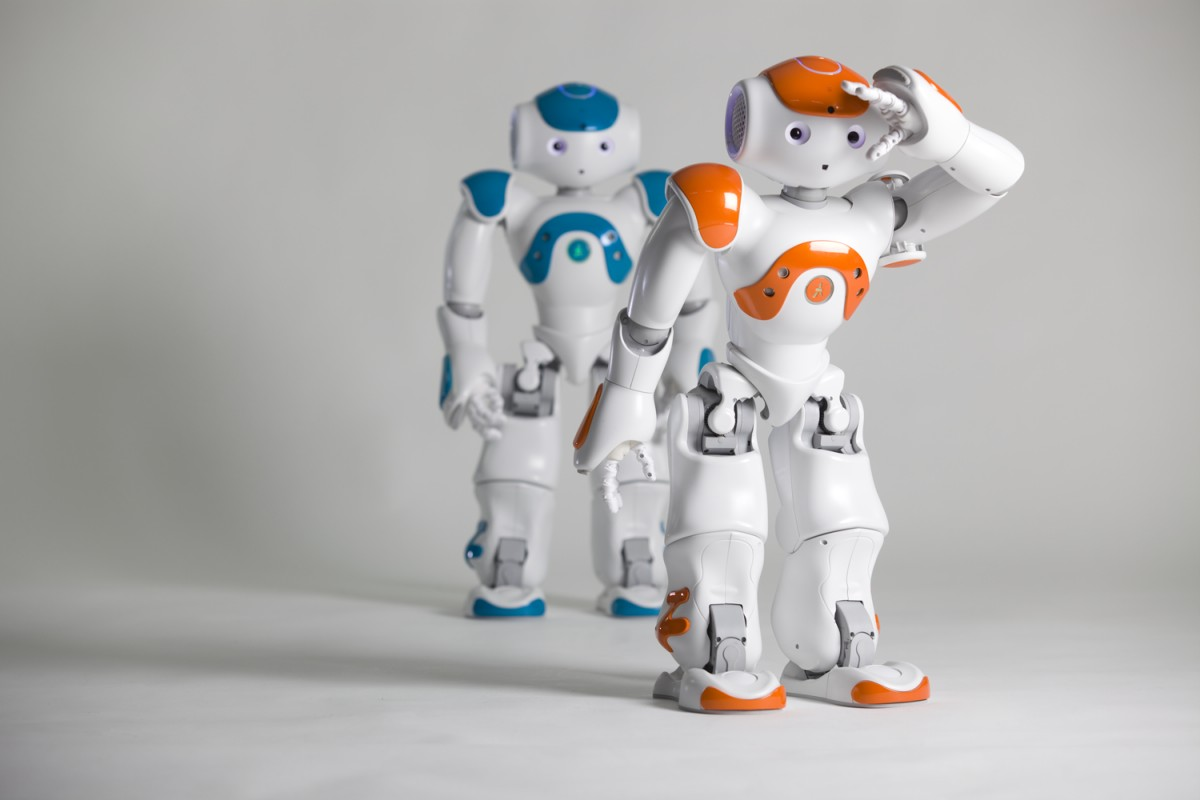
\includegraphics[width=\textwidth]{images/front.jpg}
\end{figure*}

\subsubsection*{An Artificial Intelligence project by Auke J. Wiggers, Camiel
R. Verschoor,\\Chiel Kooijman and Steven Laan}
\end{center}

\newpage

\begin{comment}
% EMPTY PAGE
\thispagestyle{empty}
\mbox{}
\newpage
\end{comment}

% OFFICIAL FRONT PAGE
\maketitle
\clearpage

% TABLE OF CONTENTS
\thispagestyle{empty}
\tableofcontents
\clearpage

\section{Introduction}
In the field of robotics, one of the main challenges is to track a robot's path
through the environment. One set of methods to tackle this problem focusses on
both creating a map of its surroundings and determining the robots position in
it, and is called Simultaneous Localisation And Mapping (SLAM). Estimating the
path is called odometry.

Some form of localisation is always needed for robots that move about freely,
to correct errors in the execution of planned actions, which are inevitable in
real-world situations. Localisation requires input from the robots sensors,
such as camera, laser range scanners, radar, sonar, or satellite navigation
systems such as GPS \citep{easton1978navigation} or GLONASS.

In this paper we focus on visual input only. This is useful because cameras are
abundant, cheap, small, light, and require little energy. Cameras are passive
sensors, which is useful when trying to avoid detection. Unlike satellite
navigation cameras work indoors given that there is enough light.
On the other hand, video input is more difficult to process, as it is subject
to lighting conditions and a single image does not provide any 3D information
by itself.

% Overview of different sections
\section{Related Work}

\section{Theory}

\section{Pipeline}
In this section, the pipeline of our proposed system is described stepwise.

\begin{figure}[!hb]
	\centerline{
		\xymatrix{
			Calibration\ar[d]\\
			Egomotion\ar[d]\\
			Reconstruction\ar[d]\\
			Modelling\ar[d]\\
			Combining Visual Odometry
		}
	}
	\caption{Schematic overview of the pipeline of the system}
	\label{fig:system}
\end{figure}

\subsection{Calibration}
Camera calibration is the process of estimating the intrinsic and extrinsic
parameters of the camera. Images taken by the Nao robot's camera are subject to
barrel distortion. Calibration provides us with camera parameters that allow us
to transform images in a way that removes the distortion.
\par
To find the camera parameters we use the method proposed by
\cite{zhang1999flexible} and implemented in the OpenCV library
\citep{opencv_library}. In this method, a chessboard-like panel of which the
dimensions are known, is held up in front of the camera in different positions.
The algorithm uses the knowledge that the panel is planar to infer the
distortion coefficients $k_1, k_2, p_1, p_2, k_3$ and camera parameters $f_x,
f_y, c_x, c_y$, forming the camera matrix:
$$
F =
\begin{bmatrix}
	f_x	& 0		& c_x\\
	0		& f_y		& c_y\\
	0		& 0		& 1\\
\end{bmatrix}
$$
The focal length (in pixels) is represented in $f_x$ and $f_y$ in the $x$- and
$y$-directions respectively. $c_x$ and $c_y$ denote the optimal camera centre
in pixels and should be near the centre of the image.


\subsection{Egomotion}
Egomotion or odometry is the process of estimating a camera's motion relative
to a rigid scene. There are two main approaches for estimating the relative
motion between two frames, namely, Image-to-Image and Image-to-World.
Image-to-Image uses two images to find a homography and reconstruct their
positions in 3D through triangulation. With Image-to-World we mean matching
points in an image to their known positions in 3D to infer the position of the
camera relative to the world coordinates.


\subsubsection{Feature extraction}
In order to create a homography between two images (Image-to-Image), or match
points of an image to a corresponding point in a 3D model (Image-to-World), we
need to recognise and match these points in different images. The descriptions
to match points (known as features or descriptors) need to be strict so that it
does not match wrong pairs, but also tolerant so that it will still match
points when conditions change. These conditions may include change of light,
change of camera position (which can result in scaling or rotation), and motion
blur. Finding descriptors also needs to be fast, so that it can be computed in
runtime.

In this section, we concisely describe the feature extraction methods that were
used in the system to extract features. In total three feature extractions
methods were applied, namely, Binary Robust Invariant Scalable Keypoints
(BRISK) \citep{Leutenegger2011}, Oriented FAST and Rotated BRIEF (ORB)
\citep{Rublee2011} and Fast Retina Keypoints (FREAK) \citep{Ortiz2012}.

\subsubsection*{Robust Invariant Scalable Keypoints}
BRISK relies on an easily configurable circular sampling pattern from which it
computes brightness comparisons to form a binary descriptor string. The unique
properties, rotation and scale invariance, of BRISK can be useful for a wide
spectrum of applications, in particular for tasks with hard real-time
constraints or limited computation power: BRISK finally offers the quality of
high-end features in such time-demanding applications.

\subsubsection*{Oriented FAST and Rotated BRIEF}
[Insert]
\subsubsection*{Fast Retina Keypoint}
[Insert]

\subsubsection{Feature Matching}
FLANN FEATUREMATCHER \citep{Muja2009}

\subsubsection{Image-to-Image}
- Match 2D with 2D descriptors.
- Normalize matches.
- Compute transformation matrices.
- Scale points.
- Find fundamental matrix and use Random Sample Consensus (RANSAC) to reject
outliers. \citep{fischler1981random}
- Compute essential matrix.
- Estimation of projection matrix.
- Decide on all candidates.

\subsubsection{Image-to-World (PnP)}
- Match 2D with 3D descriptors.
- PnP RANSAC.
- Obtain rotation matrix from rotation vector.
- Triangulate any unknown points.

\subsection{Refinement}
% We do not do refinement as our camera matrix will not change as we do not
% zoom.

\subsection{Reconstruction}
The previously described methods estimate the motion of the camera and this
pose estimation process yields the position of the different cameras in space.
The matching obtained matching feature points across frames and then estimate
the 3D position of those points in space. To obtain these 3D points there are
at least two camera poses needed to estimate the spatial position.

\subsection{Modelling}


\subsection{Multi Agent Visual Odometry}


\section{Experimental Setup}

\section{Results}

\section{Discussion}

\section{Conclusion}

\bibliographystyle{plainnat}
\bibliography{references}

\end{document}
% vim: set spell : spelllang=en_gb :
